\scanpage{5}
\mspage{1}

\uline{\inserted{Exceptional} curves of type} $(1,1)$ (over $\mathbb C$)

A) \uline{Anharmonic \inserted{elliptic} curve of square type}

Category of these curves \unsure{equivalent} : that of oriented
combinatorial squares, that is, of torsors under
\[
\mathbb Z/4\mathbb Z\simeq\mu_4(\mathbb C)\simeq
\text{group of algebraic units of }\mathbb Q[i]
\]
\margin{that is, group of units of $\mathbb Z[i]$
\unsure{ring} of integers of $\mathbb Q[i]$}

The datum of such a torsor \inserted{($S$)} allows one to twist
$\mathbb E\ell_0\overset{\mathrm{def}}\simeq
\mathbb C/\mathbb Z[i]$ and find
\[
\mathbb E\ell_0(S)\simeq\mathbb E\ell_0
\mathbin{\wedge}_{\mathbb Z/4\mathbb Z}S
\]

\margin{
\figure{
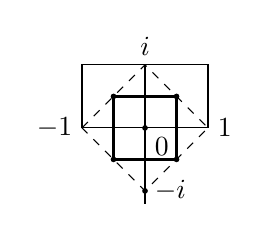
\begin{tikzpicture}[scale=.8]
\draw[thin] (-1,0)--(-1,1)--(1,1)--(1,0);
\draw[dashed] (-1,0)--(0,1)--(1,0)--(0,-1)--cycle;
\draw (-1,0)--(1,0);
\draw (0,-1.2)--(0,1);
\draw[thick] (-.5,-.5)--(-.5,.5)--(.5,.5)--(.5,-.5)--cycle;
\foreach \x/\y in {0/0,-.5/.5,.5/.5,.5/-.5,-.5/-.5,0/-1}
{\fill (\x,\y) circle (.045);}
\node[left] at (-1,0) {$-1$}; \node[right] at (1,0) {$1$};
\node[above] at (0,1) {$i$}; \node[right] at (0,-1) {$-i$};
\node[below right] at (0,0) {$0$};
\end{tikzpicture}
}}

If the square is realized as \unsure{a} \inserted{\unsure{inside|Euclidean}} square
in a Euclidean plane \inserted{$V_S$} (canonically), with centre $0$,
\deleted{
\figure{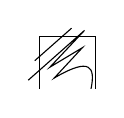
\begin{tikzpicture}[scale=.55]
\draw (0,0)--(0,1.2)--(1.3,1.2)--(1.3,0);
\draw (-.25,.2)--(1.05,1.35)--(.25,.5)--(1,.95)--(.35,.25)
 .. controls (1.2,.75) and (1.3,.5) .. (1.2,0);
\draw (-.1,.65)--(.75,1.4);
\end{tikzpicture}}
}
\figure{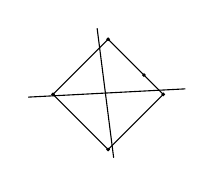
\begin{tikzpicture}[scale=.7]
\draw (-1,0)--(0,1)--(1,0)--(0,-1)--cycle;
\draw (-1.45,-.05)--(1.4,.1); \draw (.1,-1.15)--(-.2,1.2);
\foreach \x/\y in {-1/0,0/1,1/0,0/-1,.65/.35}
{\fill (\x,\y) circle (.035);}
\end{tikzpicture}}
one deduces from this in the plane (a vector space via $0$) $V_S$
a system of two \deleted{axes of}
coordinates \inserted{modulo signs}
via the diagonals, whence a
\deleted{\unsure{lattice}} \inserted{lattice}
$\Gamma_S$ in $V_S$ (discrete subgroup of
rank $2$) and
\[
\boxed{\mathbb E\ell_0(\unsure{S})\unsure{\simeq|/2|=:}
X_S=V_S/\Gamma_S}.
\]

\margin{
\figure{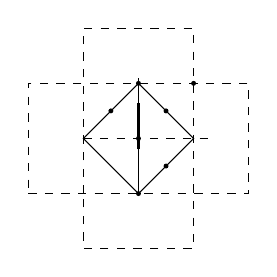
\begin{tikzpicture}[scale=.7]
\draw[dashed] (-1,-1)--(-1,2)--(1,2)--(1,-2)--(-1,-2)--(-1,-1);
\draw[dashed] (-2,-1)--(2,-1)--(2,1)--(-2,1)--cycle;
\draw (-1,0)--(0,1)--(1,0)--(0,-1)--cycle;
\draw[dashed] (-1,0)--(1.4,0);
\draw (0,-1)--(0,1.1);
\draw[very thick] (0,-.2)--(0,.65);
\foreach \x/\y in {0/0,0/1,0/-1,-.5/.5,.5/.5,.5/-.5,1/1}
{\fill (\x,\y) circle (.045);}
\end{tikzpicture}}
}

There is in $X_S$ a canonical element of order $2$
\inserted{$\unsure{\eta_S}$}
(stable under automorphisms), the other two elements of
order $2$ are interchanged by the generator $i$ of
$\mu_4(\mathbb C)\simeq\operatorname{Aut}(\unsure{X_S})$.
(\uline{Note well} $\unsure{\eta_S}$ can therefore be defined

\margin{4}
